%%%%%%%%%%%%%%%%%%%%%%%%%%%%%%%%%%%%%%%%%%%%%%%%%%%%%%%%%%%%%%%%%%%%
%% I, the copyright holder of this work, release this work into the
%% public domain. This applies worldwide. In some countries this may
%% not be legally possible; if so: I grant anyone the right to use
%% this work for any purpose, without any conditions, unless such
%% conditions are required by law.
%%%%%%%%%%%%%%%%%%%%%%%%%%%%%%%%%%%%%%%%%%%%%%%%%%%%%%%%%%%%%%%%%%%%

\documentclass{beamer}
\usetheme[faculty=science, university=uu, logo=uu-logo]{fibeamer}
\usepackage[utf8]{inputenc}
\usepackage[
  main=english %% By using `czech` or `slovak` as the main locale
                %% instead of `english`, you can typeset the
                %% presentation in either Czech or Slovak,
                %% respectively.
                %% The additional keys allow foreign texts to be
]{babel}        %% typeset as follows:
%%
%%   \begin{otherlanguage}{czech}   ... \end{otherlanguage}
%%   \begin{otherlanguage}{slovak}  ... \end{otherlanguage}
%%
%% These macros specify information about the presentation
\title{Automation of Backflow Stabilisation Parameters} %% that will be typeset on the
%\subtitle{Presentation Subtitle} %% title page.
\author{David Meadon\\
\vspace{10pt}
\footnotesize{Supervisor: Dr. C.A. Bertoglio\\
Second Assessor: Dr.Ir. B. Besselink}
}
%% These additional packages are used within the document:
\usepackage{ragged2e}  % `\justifying` text
\usepackage{booktabs}  % Tables
\usepackage{tabularx}
\usepackage{tikz}      % Diagrams
\usetikzlibrary{calc, shapes, backgrounds}
\usepackage{amsmath, amssymb}
\usepackage{url}       % `\url`s
\usepackage{listings}  % Code listings
\usepackage{graphicx,wrapfig,lipsum}  % arrange images next to text
\frenchspacing
\newcommand{\bmu}{{\textbf{u}}}
\newcommand{\bmv}{{\textbf{v}}}
\newcommand{\bmn}{{\textbf{n}}}

\newcommand{\bint}{\int\limits_{\Gamma_{N}}}
\newcommand{\fint}{\int\limits_{\Omega}}

\usepackage{physics}
\usepackage[colorinlistoftodos]{todonotes}

\usepackage{multimedia}
\usepackage{media9}
\addmediapath{./Movies/}

\usepackage{caption}
\usepackage{subcaption}
\begin{document}

 \frame{\maketitle}
 
 \AtBeginSection[]{
  \begin{frame}
  \vfill
  \centering
  \begin{beamercolorbox}[sep=8pt,center,shadow=true,rounded=true]{title}
    \usebeamerfont{title}\insertsectionhead\par%
  \end{beamercolorbox}
  \vfill
  \end{frame}
}
 
    % \AtBeginSection[]{% Print an outline at the beginning of sections
    % \begin{frame}<beamer>
    %   \frametitle{Outline for Section \thesection}
    %   \tableofcontents[currentsection]
    % \end{frame}}
 
\begin{frame}%<beamer>
  \frametitle{Outline}% for Section \thesection}
  \tableofcontents%[currentsection]
\end{frame}%}

\section{Introduction}
\subsection{Motivating Issue}
\begin{frame}{What is backflow and why does it occur?}
    Backflow is the reversal of flow along natural boundary conditions
       \begin{figure}[b]
      \centering
      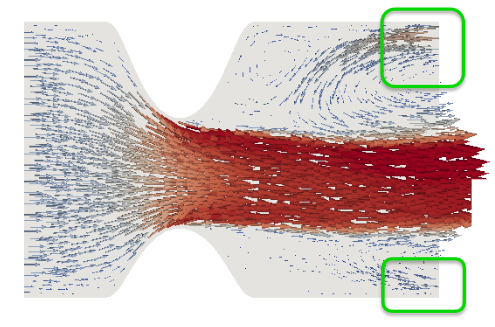
\includegraphics[width=0.6\textwidth]{Media/backflowareas.png}
  \end{figure}
\end{frame}
\begin{frame}{What is backflow and why does it occur?}
    Often occurs in physiological systems (cardiovascular, respiratory, etc)
    \begin{figure}[h]
     \centering
     \begin{subfigure}[b]{0.3\textwidth}
         \centering
         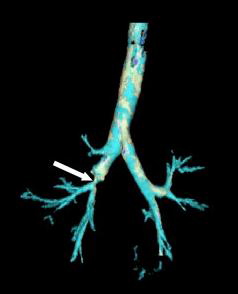
\includegraphics[width=\textwidth]{Media/Stenosis1.png}
        %  \caption{small gamma}
        %  \label{fig:smallg2}
     \end{subfigure}
     \hfill
     \begin{subfigure}[b]{0.3\textwidth}
         \centering
         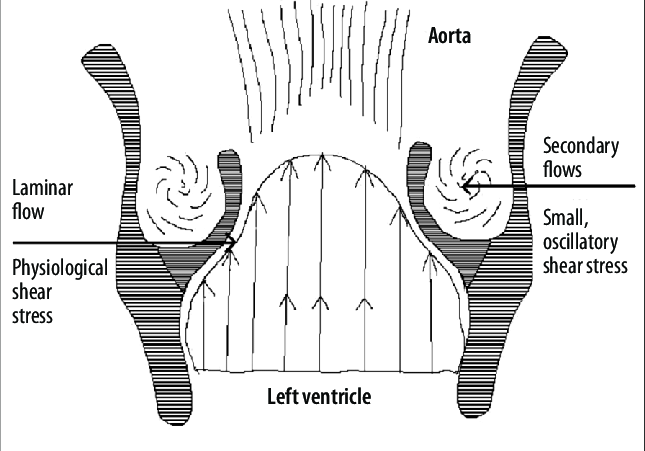
\includegraphics[width=\textwidth]{Media/Stenosis2.png}
        %  \caption{large gamma}
        %  \label{fig:highg2}
     \end{subfigure}
      \hfill
     \begin{subfigure}[b]{0.3\textwidth}
         \centering
         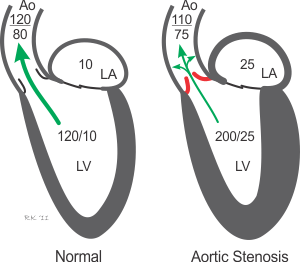
\includegraphics[width=\textwidth]{Media/Stenosis3.png}
        %  \caption{large gamma}
        %  \label{fig:highg2}
     \end{subfigure}
        % \caption{different stabilisation with different gamma's}
        % \label{fig:2 three graphs}
\end{figure}

\end{frame}
% \begin{frame}{Where does backflow occur?}
%   Some temp text
% \end{frame}
\begin{frame}{Why do we need to stabilise backflow?}
%   Would want to numerically model these physiological systems as less invasive then surgery, however 
  Regions of backflow along a boundary can cause numerical instability, resulting in incorrect solutions, wasting computational time, etc
  \begin{figure}[b]
      \centering
      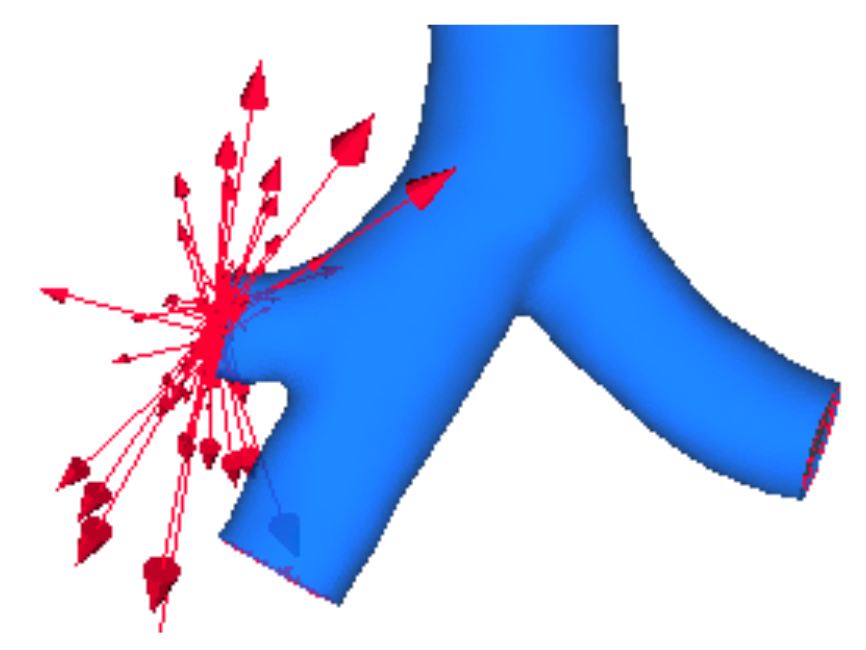
\includegraphics[width=0.4\textwidth]{Media/instability.PNG}
  \end{figure}
\end{frame}
\begin{frame}{Backflow instability example}
      \begin{center}
\includemedia[
    activate=onclick,
    % activate=pageopen,
    passcontext,
    transparent,
    width=0.75\textwidth,
]{
\includegraphics{Movies/cover.png}}{Movies/nostab.swf}
\end{center}
\end{frame}
% \begin{frame}{Mathematical foundation for backflow}

% \end{frame}
\begin{frame}{Backflow in Navier-Stokes}

\begin{block}{Navier-Stokes Equations}
\[\begin{aligned}
 \rho\partial_t\bmu + \rho(\bmu - \textbf{w})\cdot\nabla\bmu - 2\mu\nabla\cdot\epsilon(\bmu) + \nabla p &= 0 \\ \nabla\cdot\bmu &= 0 
\end{aligned}\]
\end{block}

Changing to weak form, and testing with the solution, \(\bmu\), the NS equations can be rewritten as:
\[\footnotesize
\partial_t\frac{\rho}{2}\fint\norm{\bmu}^2 = -2\mu \fint \norm{\varepsilon(\bmu)}^2 - \underbrace{\frac{\rho}{2}\bint\bmu\cdot\bmn\norm{\bmu}^2}_{\text{\huge \textasteriskcentered}}
\]


\end{frame}
\begin{frame}{Stabilising Backflow}
  
  \begin{block}{Stabilisation types}
  \begin{itemize}
      \item Velocity Penalisation:
      \(
      S = \beta\frac{\rho}{2}\bint \abs{\bmu \cdot \bmn }_- \bmu \cdot \bmv
      \)
      \item Tangential Derivative Penalisation:
      \begin{itemize}
          \item  \(      S = \gamma U_b h^2 \frac{\rho}{2} \bint \qty(t^{T}\nabla\bmu \cdot t^{T}\nabla\bmv), \qquad U_b = \max \abs{\bmu \cdot \bmn}_-\)
      \item \(
      S = \gamma\frac{\rho}{2}h^{2}\bint \abs{\bmu \cdot \bmn }_- \qty(t^{T}\nabla\bmu \cdot t^{T}\nabla\bmv)
      \)
      \end{itemize}
     
  \end{itemize}
      
  \end{block}
\end{frame}
\subsection{Problem Description}
\begin{frame}{Main Question}
\begin{center}
    \textbf{"Can these parameters be automatically chosen either at the beginning of- or during the computation such that stability is maintained while possibly improving the accuracy of the solution"}
\end{center}
\end{frame}

\section{Automation Prerequisites}

 \subsection{What are we investigating?}
    \begin{frame} {What are we investigating}
        
        \begin{block}{What is needed for automating the parameters?}
        \begin{itemize}
            \item A criterion to be met
            \item A way to test and attain that criterion
        \end{itemize}
        \end{block}
    \end{frame}
  
    \subsection{Stability Criterion}
    \begin{frame}{What do we want from the system}
        Would like the system to be dissipative.\\
        Change in energy:
        \[\footnotesize
\begin{aligned}
   \partial_t\frac{\rho}{2}\fint\norm{\bmu}^2 &= -2\mu\fint\norm{\varepsilon(\bmu)}^2 - \frac{\rho}{2}\bint\bmu\cdot\bmn\norm{\bmu}^2\\
                                              &= -\qty(2\mu\fint\norm{\varepsilon(\bmu)}^2 + \frac{\rho}{2}\bint\bmu\cdot\bmn\norm{\bmu}^2)\\
                                              &= -\qty(2\mu\fint\norm{\varepsilon(\bmu)}^2 + \frac{\rho}{2}\bint\abs{\bmu\cdot\bmn}_+\norm{\bmu}^2 - \frac{\rho}{2}\bint\abs{\bmu\cdot\bmn}_-\norm{\bmu}^2)
\end{aligned}
\]
    \end{frame}
    
    \begin{frame}{Backflow interaction}

Want the term \(B := \frac{\rho}{2}\bint\abs{\bmu\cdot\bmn}_- \bmu \cdot \bmv\) to be stabilised, so that when we test with \(\bmv = \bmu\), we get that the energy decreases, i.e. dissipation.\\
We thus need to add one of the stabilisations, and look at \(-B+S\).
    \end{frame}
    
    \begin{frame}{Stability Criterion}
    We take a very conservative approach and look only at the added stability terms to counter the instability
        \begin{block}{Stability Criterion}
            For stability, we require that the eigenvalues of \(-B+S\) in discretised form are non-negative
        \end{block}
    \end{frame}
    \subsection{Reduction of Eigenvalue Problem}
    \begin{frame}{Checking the stability criterion}
    \begin{block}{What are the problems with checking the criterion?}
        Computationally Expensive - may have to calculate the eigenvalues of a few thousand by few thousand matrix at every iteration
    \end{block}
    Idea: Don't have to consider the entire matrix
    \end{frame}
    \begin{frame}{Creating submatrix}
        Note: \(B\) is only non-zero in the presence of backflow.\\
        \(\implies B\) is exceptionally sparse when discretised.\\
        \(\implies\) Only a few small non-zero blocks\\
        \(\therefore\) We could then rather extract the block matrices of \(-B+S\) where the discretisation of \(B\) is non-zero.
        %Note that B is only non-zero in the presence of backflow so in its discretised form it is exceptionally %sparse, indeed most of the matrix is zeros besides a few small blocks.  %rewite more compact
    \end{frame}

\section{Results}
\subsection{No stabilisation}
\begin{frame}{No stabilisation}
    \begin{center}
\includemedia[
    activate=onclick,
    % activate=pageopen,
    passcontext,
    transparent,
    width=0.75\textwidth,
]{
\includegraphics{Movies/cover.png}}{NoStabilisation.swf}
\end{center}
\end{frame}
\subsection{Velocity Penalisation}
\begin{frame}{Velocity Penalisation - Eigenvalues}
Velocity Penalisation:
      \(
      S = \beta\frac{\rho}{2}\bint \abs{\bmu \cdot \bmn }_- \bmu \cdot \bmv
      \)
    \begin{center}
        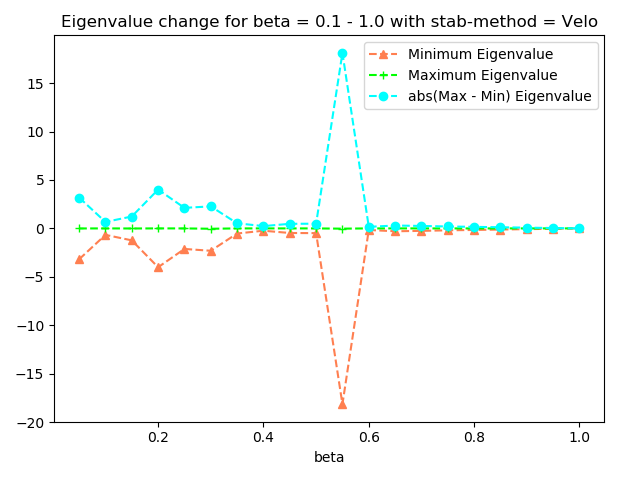
\includegraphics[width=0.8\textwidth]{Media/Beta_1_thru_0_velo.png}
    \end{center}
\end{frame}

\begin{frame}{Velocity Penalisation - Min Eigenvalue}
Velocity Penalisation:
      \(
      S = \beta\frac{\rho}{2}\bint \abs{\bmu \cdot \bmn }_- \bmu \cdot \bmv
      \)
    \begin{center}
        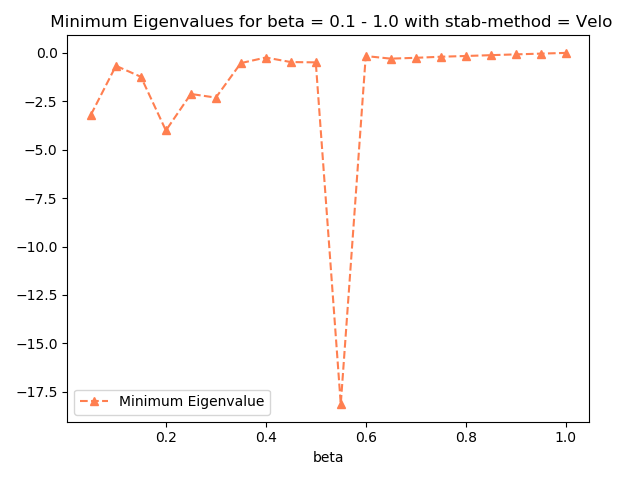
\includegraphics[width=0.8\textwidth]{Media/Beta_1_thru_0_velo_min.png}
    \end{center}
\end{frame}

\subsection{Tangential Penalisation Max}
% \begin{frame}{Change in eigenvalues over time}
%         \begin{center}
% \includemedia[
%     activate=onclick,
%     % activate=pageopen,
%     passcontext,
%     transparent,
%     width=0.75\textwidth,
% ]{
\includegraphics{Movies/cover.png}}{NoStabilisation.swf}
% \end{center}
% \end{frame}
\begin{frame}{Tang. Penalisation Max - Eigenvalues - Small Gamma}
Tang. Penal. Max: \(      S = \gamma U_b h^2 \frac{\rho}{2} \bint \qty(t^{T}\nabla\bmu \cdot t^{T}\nabla\bmv),  ~~U_b = \max \abs{\bmu \cdot \bmn}_-\)
    \begin{center}
        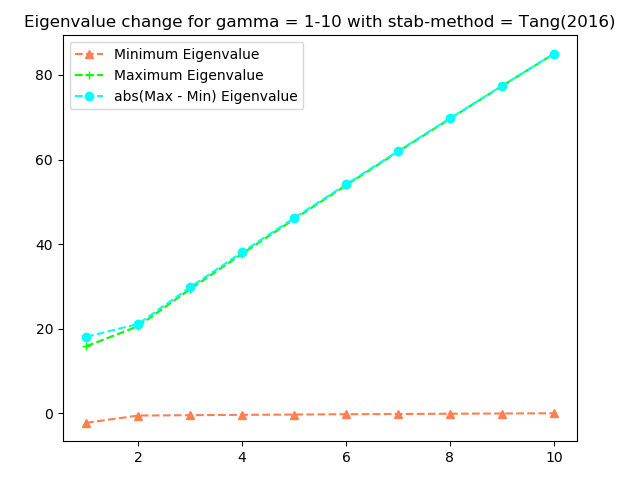
\includegraphics[width=0.8\textwidth]{Media/Gamma_1_thru_10_tang(2016).png}
    \end{center}
\end{frame}

\begin{frame}{Tang. Penalisation Max - Min Eigenvalues - Small Gamma}
Tang. Penal. Max: \(      S = \gamma U_b h^2 \frac{\rho}{2} \bint \qty(t^{T}\nabla\bmu \cdot t^{T}\nabla\bmv),  ~~U_b = \max \abs{\bmu \cdot \bmn}_-\)
    \begin{center}
        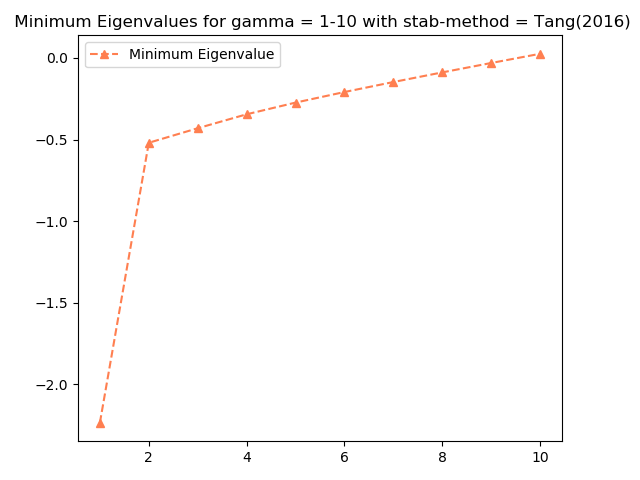
\includegraphics[width=0.8\textwidth]{Media/Gamma_1_thru_10_tang(2016)_min.png}
    \end{center}
\end{frame}

\begin{frame}{Tang. Penalisation Max - Eigenvalues - Large Gamma}
Tang. Penal. Max: \(      S = \gamma U_b h^2 \frac{\rho}{2} \bint \qty(t^{T}\nabla\bmu \cdot t^{T}\nabla\bmv),  ~~U_b = \max \abs{\bmu \cdot \bmn}_-\)
    \begin{center}
        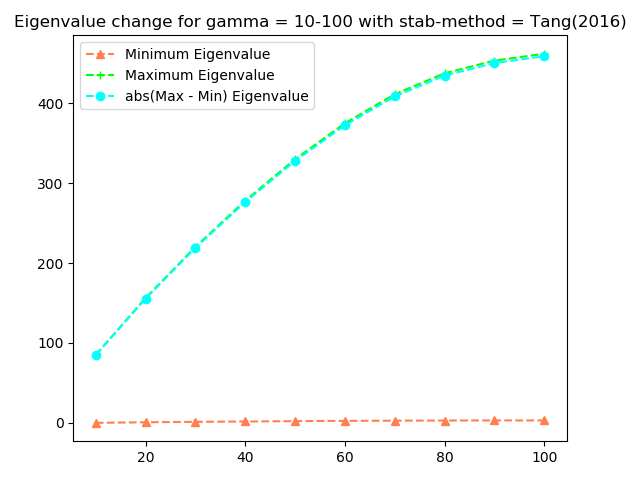
\includegraphics[width=0.8\textwidth]{Media/Gamma_10_thru_100_tang(2016).png}
    \end{center}
\end{frame}

\begin{frame}{Tang. Penalisation Max - Min Eigenvalues - Large Gamma}
Tang. Penal. Max: \(      S = \gamma U_b h^2 \frac{\rho}{2} \bint \qty(t^{T}\nabla\bmu \cdot t^{T}\nabla\bmv),  ~~U_b = \max \abs{\bmu \cdot \bmn}_-\)
    \begin{center}
        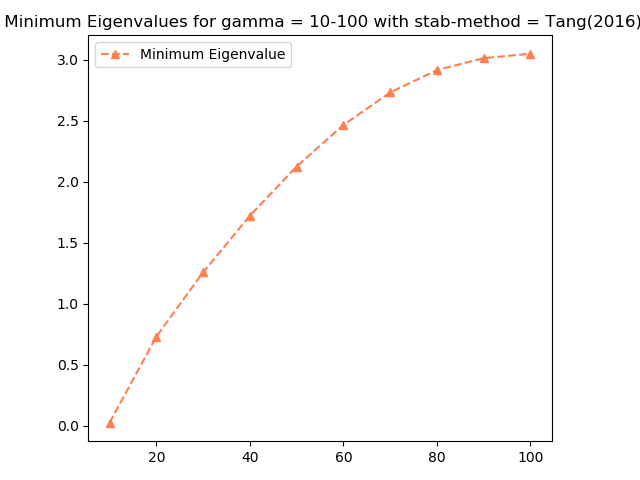
\includegraphics[width=0.8\textwidth]{Media/Gamma_10_thru_100_tang(2016)_min.png}
    \end{center}
\end{frame}

\begin{frame}{Tang. Penalisation Max - Test}
    \begin{center}
\includemedia[
    activate=onclick,
    % activate=pageopen,
    passcontext,
    transparent,
    width=0.75\textwidth,
]{
\includegraphics{Movies/cover.png}}{BFS4G100.swf}
\end{center}
\end{frame}

\subsection{Tangential Penalisation}
\begin{frame}{Tang. Penalisation - Eigenvalues - Small Gamma}
    Tang. Penalisation: \(
      S = \gamma\frac{\rho}{2}h^{2}\bint \abs{\bmu \cdot \bmn }_- \qty(t^{T}\nabla\bmu \cdot t^{T}\nabla\bmv)
      \)
    \begin{center}
        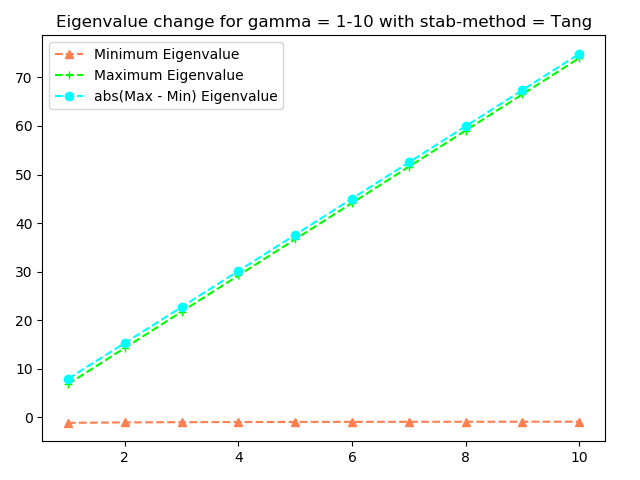
\includegraphics[width=0.8\textwidth]{Media/Gamma_1_thru_10_tang.png}
    \end{center}
\end{frame}

\begin{frame}{Tang. Penalisation - Min Eigenvalues - Small Gamma}
    Tang. Penalisation: \(
      S = \gamma\frac{\rho}{2}h^{2}\bint \abs{\bmu \cdot \bmn }_- \qty(t^{T}\nabla\bmu \cdot t^{T}\nabla\bmv)
      \)
    \begin{center}
        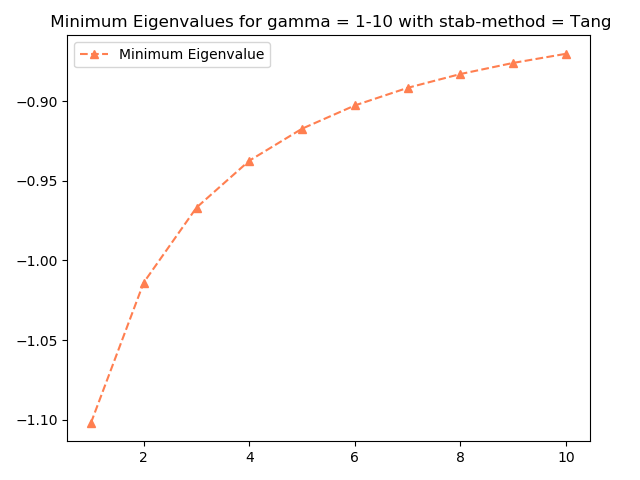
\includegraphics[width=0.8\textwidth]{Media/Gamma_1_thru_10_tang_min.png}
    \end{center}
\end{frame}

\begin{frame}{Tang. Penalisation - Eigenvalues - Large Gamma}
    Tang. Penalisation: \(
      S = \gamma\frac{\rho}{2}h^{2}\bint \abs{\bmu \cdot \bmn }_- \qty(t^{T}\nabla\bmu \cdot t^{T}\nabla\bmv)
      \)
    \begin{center}
        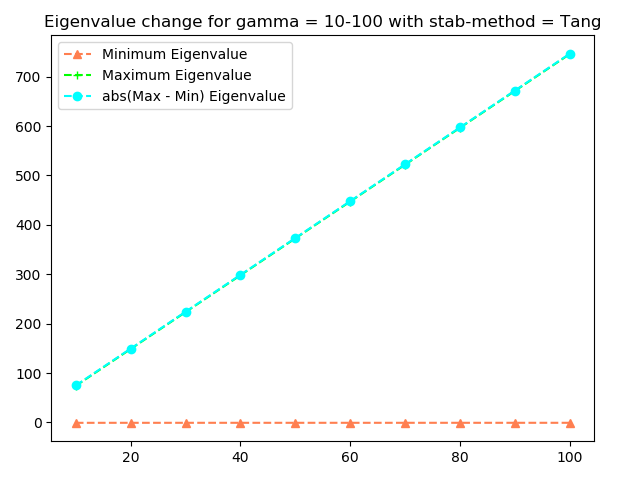
\includegraphics[width=0.8\textwidth]{Media/Gamma_10_thru_100_tang.png}
    \end{center}
\end{frame}

\begin{frame}{Tang. Penalisation - Min Eigenvalues - Large Gamma}
    Tang. Penalisation: \(
      S = \gamma\frac{\rho}{2}h^{2}\bint \abs{\bmu \cdot \bmn }_- \qty(t^{T}\nabla\bmu \cdot t^{T}\nabla\bmv)
      \)
    \begin{center}
        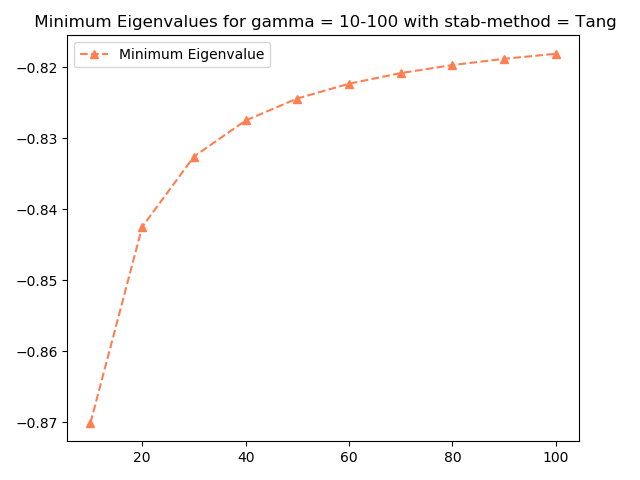
\includegraphics[width=0.8\textwidth]{Media/Gamma_10_thru_100_tang_min.png}
    \end{center}
\end{frame}

\begin{frame}{Tang. Penalisation - Test}
    \begin{center}
\includemedia[
    activate=onclick,
    % activate=pageopen,
    passcontext,
    transparent,
    width=0.75\textwidth,
]{
\includegraphics{Movies/cover.png}}{BFS3G100.swf}
\end{center}
\end{frame}

\section{Conclusion}
    \begin{frame}{Conclusion}
        \begin{itemize}
            \item Backflow can change at every time-step, so cannot automate the parameter at the beginning of the computation to be lower than the already found stable values.
            \item Tang. Penalisation Max will have stability for a large enough gamma, irrespective of any other stabilising terms.
            \item Tang. Penalisation cannot stabilise by itself, for any value of gamma, and may rely on other stabilising terms to prevent instability.
            \item Similarly, below \(\beta = 1\), the Velocity Penalisation cannot prevent instability by itself
        \end{itemize}    
    \end{frame}
    
    \begin{frame}{Whats more to be considered?}
    \begin{itemize}
        \item Try to understand why the Tang. Penalisation will not be stabilised for a large enough gamma.
        \item Try to include the other stabilising terms, such as viscosity.
    \end{itemize}
        
    \end{frame}

    
    \begin{frame}{}
        \begin{center}
            \huge \textbf{Questions?}
        \end{center}
    \end{frame}

%  

%   \AtBeginSection[]{% Print an outline at the beginning of sections
%     \begin{frame}<beamer>
%       \frametitle{Outline for Section \thesection}
%       \tableofcontents[currentsection]
%     \end{frame}}

%     \section{Light Frames}
%     \subsection{Blind Text}
%     \begin{frame}{Jabberwocky}
%       \framesubtitle{Lewis Carroll}%
%       \begin{tikzpicture}[overlay,remember picture]
%         \node[anchor=south east,xshift=-30pt,yshift=35pt]
%           at (current page.south east) {
%             \includegraphics[width=35mm]{resources/jabberwocky-light}
%           };
%       \end{tikzpicture}%
%       'Twas brillig, and the slithy toves\\
%       Did gyre and gimble in the wabe;\\
%       All mimsy were the borogoves,\\
%       And the mome raths outgrabe.\\\bigskip

%       “Beware the Jabberwock, my son!\\
%       The jaws that bite, the claws that catch!\\
%       Beware the Jubjub bird, and shun\\
%       The frumious Bandersnatch!”\\
%     \end{frame}

%     \begin{frame}[label=lists]{Lists and locales}
%       \framesubtitle{Lorem ipsum dolor sit amet}
%       \begin{columns}[onlytextwidth]
%         \column{.5\textwidth}
%           \begin{itemize}
%             \item Nulla nec lacinia odio. Curabitur urna tellus.
%             \begin{itemize}
%               \item Fusce id sodales dolor. Sed id metus dui.
%               \begin{itemize}
%                 \item Cupio virtus licet mi vel feugiat.
%               \end{itemize}
%             \end{itemize}
%           \end{itemize}
%         \column{.5\textwidth}
%           \begin{enumerate}
%             \item Donec porta, risus porttitor egestas scelerisque video.
%             \begin{enumerate}
%               \item Nunc non ante fringilla, manus potentis cario.
%               \begin{enumerate}
%                 \item Pellentesque servus morbi tristique.
%               \end{enumerate}
%             \end{enumerate}
%           \end{enumerate}
%       \end{columns}
%       \bigskip
%       \justifying

%       {\uselanguage{czech}Nechť již hříšné saxofony ďáblů
%       rozzvučí síň úděsnými tóny waltzu, tanga a quickstepu!}
%       {\uselanguage{slovak} Nezvyčajné kŕdle šťastných figliarskych
%       ďatľov učia pri kótovanom ústí Váhu mĺkveho koňa Waldemara
%       obžierať väč\-šie kusy exkluzívnej kôry.}
%       {\uselanguage{english}The quick, brown fox jumps over a lazy
%       dog. DJs flock by when MTV ax quiz prog. “Now fax quiz Jack!”}
%     \end{frame}

%     \subsection{Structuring Elements}
%     \begin{frame}[label=simmonshall]{Text blocks}
%       \framesubtitle{In plain, example, and \alert{alert} flavour}
%       \alert{This text} is highlighted.

%       \begin{block}{A plain block}
%         This is a plain block containing some \alert{highlighted text}.
%       \end{block}
%       \begin{exampleblock}{An example block}
%         This is an example block containing some \alert{highlighted text}.
%       \end{exampleblock}
%       \begin{alertblock}{An alert block}
%         This is an alert block containing some \alert{highlighted text}.
%       \end{alertblock}
%     \end{frame}

%     \begin{frame}[label=proof]{Definitions, theorems, and proofs}
%       \framesubtitle{All integers divide zero}
%       \begin{definition}
%         $\forall a,b\in\mathds{Z}: a\mid b\iff\exists c\in\mathds{Z}:a\cdot c=b$
%       \end{definition}
%       \begin{theorem}
%         $\forall a\in\mathds{Z}: a\mid 0$
%       \end{theorem}
%       \begin{proof}[Proof\nopunct]
%         $\forall a\in\mathds{Z}: a\cdot 0=0$
%       \end{proof}
%     \end{frame}

%     \subsection{Numerals and Mathematics}
%     \begin{frame}[label=math]{Numerals and Mathematics}
%       \framesubtitle{Formulae, equations, and expressions}
%       \begin{columns}[onlytextwidth]
%         \column{.20\textwidth}
%           1234567890
%         \column{.20\textwidth}
%           \oldstylenums{1234567890}
%         \column{.20\textwidth}
%           $\hat{x}$, $\check{x}$, $\tilde{a}$,
%           $\bar{a}$, $\dot{y}$, $\ddot{y}$
%         \column{.40\textwidth}
%           $\int \!\! \int f(x,y,z)\,\mathsf{d}x\mathsf{d}y\mathsf{d}z$
%       \end{columns}
%       \begin{columns}[onlytextwidth]
%         \column{.5\textwidth}
%           $$\frac{1}{\displaystyle 1+
%             \frac{1}{\displaystyle 2+
%             \frac{1}{\displaystyle 3+x}}} +
%             \frac{1}{1+\frac{1}{2+\frac{1}{3+x}}}$$
%         \column{.5\textwidth}
%           $$F:\left| \begin{array}{ccc}
%           F''_{xx} & F''_{xy} &  F'_x \\
%           F''_{yx} & F''_{yy} &  F'_y \\
%           F'_x     & F'_y     & 0
%           \end{array}\right| = 0$$
%       \end{columns}
%       \begin{columns}[onlytextwidth]
%         \column{.3\textwidth}
%           $$\mathop{\int \!\!\! \int}_{\mathbf{x} \in \mathds{R}^2}
%           \! \langle \mathbf{x},\mathbf{y}\rangle\,\mathsf{d}\mathbf{x}$$
%         \column{.33\textwidth}
%           $$\overline{\overline{a\alpha}^2+\underline{b\beta}
%           +\overline{\overline{d\delta}}}$$
%         \column{.37\textwidth}
%           $\left] 0,1\right[ + \lceil x \rfloor - \langle x,y\rangle$
%       \end{columns}
%       \begin{columns}[onlytextwidth]
%         \column{.4\textwidth}
%           \begin{eqnarray*}
%           e^x &\approx& 1+x+x^2/2! + \\
%              && {}+x^3/3! + x^4/4!
%           \end{eqnarray*}
%         \column{.6\textwidth}
%           $${n+1\choose k} = {n\choose k} + {n \choose k-1}$$
%       \end{columns}
%     \end{frame}

%     \subsection{Figures and Code Listings}
%     \begin{frame}[label=figs1]{Figures}
%       \framesubtitle{Tables, graphs, and images}
%       \begin{table}[!b]
%         {\carlitoTLF % Use monospaced lining figures
%         \begin{tabularx}{\textwidth}{Xrrr}
%           \textbf{Faculty} & \textbf{With \TeX} & \textbf{Total} &
%           \textbf{\%} \\
%           \toprule
%           Faculty of Informatics       & 1\,716  & 2\,904  &
%           59.09 \\% 1433
%           Faculty of Science           & 786     & 5\,275  &
%           14.90 \\% 1431
%           Faculty of $\genfrac{}{}{0pt}{}{\textsf{Economics and}}{%
%           \textsf{Administration}}$    & 64      & 4\,591  &
%           1.39  \\% 1456
%           Faculty of Arts              & 69      & 10\,000 &
%           0.69  \\% 1421
%           Faculty of Medicine          & 8       & 2\,014  &
%           0.40  \\% 1411
%           Faculty of Law               & 15      & 4\,824  &
%           0.31  \\% 1422
%           Faculty of Education         & 19      & 8\,219  &
%           0.23  \\% 1441
%           Faculty of Social Studies    & 12      & 5\,599  &
%           0.21  \\% 1423
%           Faculty of Sports Studies    & 3       & 2\,062  &
%           0.15  \\% 1451
%           \bottomrule
%         \end{tabularx}}
%         \caption{The distribution of theses written using \TeX\ during 2010--15 at MU}
%       \end{table}
%     \end{frame}
%     \begin{frame}[label=figs2]{Figures}
%       \framesubtitle{Tables, graphs, and images}
%       \begin{figure}[b]
%         \centering
%         % Flipping a coin
%         % Author: cis
%         \tikzset{
%           head/.style = {fill = none, label = center:\textsf{H}},
%           tail/.style = {fill = none, label = center:\textsf{T}}}
%         \scalebox{0.65}{\begin{tikzpicture}[
%             scale = 1.5, transform shape, thick,
%             every node/.style = {draw, circle, minimum size = 10mm},
%             grow = down,  % alignment of characters
%             level 1/.style = {sibling distance=3cm},
%             level 2/.style = {sibling distance=4cm},
%             level 3/.style = {sibling distance=2cm},
%             level distance = 1.25cm
%           ]
%           \node[shape = rectangle,
%             minimum width = 6cm, font = \sffamily] {Coin flipping}
%           child { node[shape = circle split, draw, line width = 1pt,
%                   minimum size = 10mm, inner sep = 0mm, rotate = 30] (Start)
%                   { \rotatebox{-30}{H} \nodepart{lower} \rotatebox{-30}{T}}
%           child {   node [head] (A) {}
%              child { node [head] (B) {}}
%              child { node [tail] (C) {}}
%           }
%           child {   node [tail] (D) {}
%              child { node [head] (E) {}}
%              child { node [tail] (F) {}}
%           }
%           };

%           % Filling the root (Start)
%           \begin{scope}[on background layer, rotate=30]
%             \fill[head] (Start.base) ([xshift = 0mm]Start.east) arc (0:180:5mm)
%               -- cycle;
%             \fill[tail] (Start.base) ([xshift = 0pt]Start.west) arc (180:360:5mm)
%               -- cycle;
%           \end{scope}

%           % Labels
%           \begin{scope}[nodes = {draw = none}]
%             \path (Start) -- (A) node [near start, left]  {$0.5$};
%             \path (A)     -- (B) node [near start, left]  {$0.5$};
%             \path (A)     -- (C) node [near start, right] {$0.5$};
%             \path (Start) -- (D) node [near start, right] {$0.5$};
%             \path (D)     -- (E) node [near start, left]  {$0.5$};
%             \path (D)     -- (F) node [near start, right] {$0.5$};
%             \begin{scope}[nodes = {below = 11pt}]
%               \node [name = X] at (B) {$0.25$};
%               \node            at (C) {$0.25$};
%               \node [name = Y] at (E) {$0.25$};
%               \node            at (F) {$0.25$};
%             \end{scope}
%           \end{scope}
%         \end{tikzpicture}}
%         \caption{Tree of probabilities -- Flipping a coin\footnote[frame]{%
%           A derivative of a diagram from \url{texample.net} by cis, CC BY 2.5 licensed}}
%       \end{figure}
%     \end{frame}

%     \defverbatim[colored]\sleepSort{
%       \begin{lstlisting}[language=C,tabsize=2]
%   #include <stdio.h>
%   #include <unistd.h>
%   #include <sys/types.h>
%   #include <sys/wait.h>

%   // This is a comment
%   int main(int argc, char **argv)
%   {
%           while (--c > 1 && !fork());
%           sleep(c = atoi(v[c]));
%           printf("%d\n", c);
%           wait(0);
%           return 0;
%   }
%     \end{lstlisting}}
%     \begin{frame}{Code listings}{An example source code in C}
%       \sleepSort
%     \end{frame}

%     \subsection{Citations and Bibliography}
%     \begin{frame}[label=citations]{Citations}
%       \framesubtitle{\TeX, \LaTeX, and Beamer}

%       \justifying\TeX\ is a programming language for the typesetting
%       of documents. It was created by Donald Erwin Knuth in the late
%       1970s and it is documented in \emph{The \TeX
%       book}~\cite{knuth84}.

%       In the early 1980s, Leslie Lamport created the initial version
%       of \LaTeX, a high-level language on top of \TeX, which is
%       documented in \emph{\LaTeX : A Document Preparation
%       System}~\cite{lamport94}. There exists a healthy ecosystem of
%       packages that extend the base functionality of \LaTeX;
%       \emph{The \LaTeX\ Companion}~\cite{MG94} acts as a guide
%       through the ecosystem.

%       In 2003, Till Tantau created the initial version of Beamer, a
%       \LaTeX\ package for the creation of presentations. Beamer is
%       documented in the \emph{User's Guide to the Beamer
%       Class}~\cite{tantau04}.
%     \end{frame}

%     \begin{frame}[label=bibliography]{Bibliography}
%       \framesubtitle{\TeX, \LaTeX, and Beamer}
%       \begin{thebibliography}{9}
%         \bibitem{knuth84}
%             Donald~E.~Knuth.
%             \emph{The \TeX book}.
%             Addison-Wesley, 1984.
%         \bibitem{lamport94}
%             Leslie~Lamport.
%             \emph{\LaTeX : A Document Preparation System}.
%             Addison-Wesley, 1986.
%         \bibitem{MG94}
%             M.~Goossens, F.~Mittelbach, and A.~Samarin.
%             \emph{The \LaTeX\ Companion}.
%             Addison-Wesley, 1994.
%         \bibitem{tantau04}
%             Till~Tantau.
%             \emph{User's Guide to the Beamer Class Version 3.01}.
%             Available at \url{http://latex-beamer.sourceforge.net}.
%         \bibitem{MS05}
%             A.~Mertz and W.~Slough.
%             Edited by B.~Beeton and K.~Berry.
%             \emph{Beamer by example} In TUGboat,
%               Vol. 26, No. 1., pp. 68-73.
%       \end{thebibliography}
%     \end{frame}

 
%  % \begin{frame}{This is where you start}
%     Add your frames below this and then I'll sort out the format later
% \end{frame}

%\AtBeginSection[]{% Print an outline at the beginning of sections
    \begin{frame}%<beamer>
      \frametitle{Outline}% for Section \thesection}
      \tableofcontents%[currentsection]
    \end{frame}%}
    
    \section{Introduction}
    \subsection{Motivating Problem}
    \begin{frame}{Motivating Problem}
      \includegraphics[scale=0.4]{resources/Molly.PNG}
    \end{frame}
    \subsection{Problem Description}
    \begin{frame}{Main Question}
    \begin{center}
        \textbf{"To What Extent Should Content in Social Media be Filtered?"}
    \end{center}
    \begin{block}{Sub-questions}
        \begin{enumerate}
       \item What content should be filtered?
       \item Who should carry out the regulation?
       \item How effective are filters?
       \end{enumerate}
       \end{block}
    \end{frame}
    
    \section{Main Part} %%   CHANGE THIS NAME
    \subsection{What content should be filtered?}
    \begin{frame} {What content should be filtered?}
 
        \begin{block}{Why is this sub-question relevant?}
        \begin{itemize}
            \item To narrow down the scope
        \end{itemize}
        \end{block}
        \begin{block} {To be examined:}
        \begin{itemize}
          \item Copy-righted content 
          \item Terrorism content    
          \item Self-harm content   

           \end{itemize}
        \end{block}
    \end{frame}
  
    \subsection{Who should carry out the regulation?}
    \begin{frame}{Who should carry out the regulation?}

        \begin{block}  {Why is this sub-question relevant?}
        \begin{itemize}
            \item To determine the level of conflicts (micro,meso,macro)
        \end{itemize}
        \end{block}
        
        \begin{block} {What parties are involved} 
        \begin{itemize}
            \item Users
            \item Social Media Providers (Facebook, Instagram, etc)
            \item Governments
            %\item Academics
            % Can refer: The next subquestion we will examine is~. THis subquestion is toward to the main question because we can determine the level of conflicts for example, individual, social media providers and governments. we can ask question If harmful contents or hate speech on social media caused physical harm who should get responsibility. Individual, social media providers, goverments. the reason why they have responsibility and what is downside if the duty performed only by individual and provider.-> we need law-> government need to engage in regulating at some lever.
        \end{itemize}
        \end{block}

    \end{frame}
    \subsection{How effective are filters?}
    \begin{frame}{How effective are filters?}
    \begin{block}{Why is this sub-question relevant?}
        \begin{itemize}
                \item How Viable are they to Implement
                \item Their Actual Effectiveness in Blocking Specific Content %% both kind of similar
            \end{itemize}
      \end{block}
      
      \begin{block}{What we will consider}
        \begin{itemize}
                \item Comparison of Different Filtering Techniques (DNS Poisoning, IP Packet Filtering and URL Blocking) 
                \item Over-Blocking vs. Under-Blocking
                \item Circumventing Filtering
            \end{itemize}
      \end{block}
    \end{frame}
    

 
    
    \section{Conclusion}
    \subsection{Conclusion}
    \begin{frame}{Conclusion}
    %first sub:from the view point of consequentilist, we shouldn't enhance regulation for copyrighted contents but should filter extremist contents. however deontological view shows that we should filter both. second sub:They all have responsibilities according to  deontology, however we can't avoid regulating conducted by government.  so the our answer to main question is~
    \begin{block}{Content to always be filtered}
    \begin{itemize}
        \item Explicit content regarding death or injury
        \item Terrorist Activity
        \item More generally content that directly harms people's lives
    \end{itemize}
    \end{block}
    
    All other content should only be blocked if the algorithm can filter it with enough accuracy.
        
    \end{frame}
    \begin{frame}[label=bibliography]{Bibliography}
    \footnotesize
      %\framesubtitle{\TeX, \LaTeX, and Beamer}
      \begin{thebibliography}{9}
        \bibitem{knuth84}
             T.~Hughes.
            \emph{“Instagram helps girls self-harm”} In Daily Star.
          Sep. 2018. [Online]. Available at \url{https://www.dailystar.co.uk/real-life/728459/Instagram-helps-girls-self-harm.}
        \bibitem{lamport94}
              T. Heyman, 
              \emph{“EU plans new laws to target terror on social media sites”},The  National,Aug.  2018.  [Online].  Available at \url{https://www.thenational.ae/world/europe/eu-plans-new-laws-to-target-terror-on-social-media-sites-1.762013}
        \bibitem{MG94}
            H. T.Tavani,
            \emph{Ethics and Technology: Controversies, Questions, and Strategies for Ethical Computing, fourth.}
            Wiley, 2012,isbn: 9781118281727.
        \bibitem{tantau04}
            C.  D.  Hunter, 
            \emph{“Internet  filter  effectiveness  -  testing  over-  and  underinclusive  blockingdecisions  of  four  popular  web  filters”}
            ,Social  Science  Computer  Review,  vol.  18,  no.  2,pp. 214–222, 2000. doi: \url{https://doi.org/10.1177/089443930001800209}
        %\bibitem{MS05}
         %    LexisNexisR©,
          %   \emph{Survey  of  Law  Enforcement  Personnel  and  Their  Use  of  Social  Media,}
           %  LexisNexisR©Risk Solutions, 2014. [Online]. Available at \url{www.lexisnexis.com/investigations.}
      \end{thebibliography}
    \end{frame}
    
    \begin{frame}{}
        \begin{center}
            \huge \textbf{Questions?}
        \end{center}
    \end{frame}
    

\end{document}
